\documentclass[12pt]{article}
\usepackage[utf8]{inputenc}

\usepackage{mystyle}
\usepackage{parskip}
\usepackage{float}
\usepackage[normalem]{ulem}

% Comic Sans
% \usepackage{sansmathfonts}
% \usepackage{fontspec}
% \setmainfont{Comic Sans MS}

% \usepackage{fontspec}
% \setmainfont{Wingdings-Regular.ttf}

% \usepackage{libertine}

% fancy header
\usepackage{fancyhdr}
\pagestyle{fancy}
\rhead{Joseph Sullivan}

\title{Variations of Hodge Structures}
\author{Joseph Sullivan}
\date{April 2024}

\newcommand{\reg}{\mathrm{reg}}
\newcommand{\sing}{\mathrm{sing}}
\newcommand{\Pic}{\mathrm{Pic}}
\newcommand{\sgn}{\mathrm{sgn}}
\newcommand{\FS}{\mathrm{FS}}
\newcommand{\Alb}{\mathrm{Alb}}
\newcommand{\CMan}{\text{$\C$-$\mathsf{Man}$}}

\newcommand{\ev}{\mathrm{ev}}

\newcommand{\Hol}{\mathrm{Hol}}

\begin{document}

\maketitle

\section{Motivation}

\begin{thm}[Ehresmann]
    Let $\cX\xrightarrow{\phi} B$ be a family of complex manifolds, i.e., a holomorphic proper submersion. Let $0\in B$. Then, up to replacing $B$ with a neighborhood of $0$, there exists a $C^\infty$ trivialization
    \begin{cd}
        \cX \ar[rr,"(T_0{,}\phi)"] \ar[dr,"\phi"'] & & X_0\times B \ar[dl,"\mathrm{pr}_2"]\\
         & B & 
    \end{cd}
    % such that the fibers of $T_0$ (i.e., horizontal) are complex submanifolds of $\cX$.
\end{thm}

In other words, families/proper submersions are $C^\infty$ fiber products.

\begin{proof}[Proof sketch.]
    In a contractible neighborhood of $B$, choose a vector field whose flow gives a deformation retraction to $0$. Lift this vector field upstairs (non uniquely) and the flow gives a deformation retraction onto the fiber to $X_0$. The flow exists for long enough due to properness.
\end{proof}

\begin{rmk}
    \textbf{Fibers only diffeomorphic, not biholomorphic.} We can understand these diffeomorphisms as equipping our favorite fiber $X_0$ with different complex structures, which will then induce different Hodge decompositions, i.e., different Hodge structures on cohomology.
\end{rmk}

Starting with a family, we want to extract just the notion of how the Hodge structures vary. So, we throw away this fiber product and replace it with a filtration of vector bundles over the base. That is, we will attach the de Rham cohomology of $X_b$ to $b\in B$ to get our largest vector bundle, and then we will have subbundles which are attaching the $p$th Hodge filtration to $b$.


\newpage
\section{Formalism}

\begin{defn}
    A local system $H$ over $B$ is a sheaf of abelian groups locally isomorphic to a constant sheaf of stalk $G$.
\end{defn}

We will call an isomorphism $H|_U \cong \underline{G}|_U$ a trivialization of the local system.

\begin{prop}
    Let $\pi: \cX \to B$ be a family of complex manifolds. Then, $R^k\pi_* \underline{\C}$ is a local system on $B$.
\end{prop}

\begin{proof}
    One can check that $R^k\pi_* \underline{\C}$ is the sheafification of
    \[U\mapsto H^k(\pi^{-1}(U), \underline{\C}).\]
    (by arguing that $\cF \mapsto s H^k(\pi^{-}(-),\cF)$ is a universal $\delta$-functor because it vanishes on injective objects, and then constructing a morphism of $\delta$-functors from it to $R^k\pi_*$ that agrees on degree 0).

    Then, at a point $0\in B$, by Ehresmann's theorem there exists a (contractible) neighborhood $B_0$ such that $\pi^{-1}(B_0)$ is $X_0\times B_0$, so projection $X_0\times B_0\to X_0$ is a homotopy equivalence, so
    \[H^k(X_0\times B_0, \C) \cong H^k(X_0,\C).\]
    This will tell us
    \[(R^k\pi_* \underline\C)|_{U_0} \cong \underline{H^k(X_0,\C)}|_{U_0}\]
    which tells us that it is indeed a local system on $B$.
\end{proof}

Note that $R^k\pi_* \underline{\C}$ and local systems in general are \textit{not} exactly vector bundles, in the sense of being locally free $\cO_B$ or $C^\infty$ modules. Instead, we only have ``flat'' sections, sections which are constant on the trivializations of the local system.

\begin{defn}
    The holomorphic vector bundle associated to a $\C$-vector space local system $H$ on $B$ is
    \[\cH = H \otimes_\C \cO_B.\]
    We denote the locally free sheaf by $\cH$ and the geometric vector bundle by $\bH$. This vector bundle comes equipped with the holomorphic connection $\nabla$ called the \textbf{Gauss-Manin connection}, defined as follows: for $\sigma\in \cH(U)$, write locally $\sigma = \sum_i \alpha_i \sigma_i$ where $\sigma_i$ form a basis of a local trivialization of $H$, and define
    \begin{align*}
        \nabla: \cH &\longrightarrow \cH \otimes \Omega_B\\
        \sigma &\longmapsto \sum_{i} \sigma_i \otimes d \alpha_i.
    \end{align*}
    This is well-defined, since the transition functions $g_{ij}: U_{ij}\to \GL(\C^r)$ are constant because $\cH$ comes from the local system $H$.
\end{defn}

This Gauss-Manin connection is flat, in the sense that $\Theta = \nabla \circ \nabla = 0$, since the Gauss-Manin connection is computed locally by taking exterior derivatives of component functions of flat sections, and $d^2=0$.

We can also study a local system by its obstruction to being constant, which is the way in which $\pi_1(B)$ ``moves'' sections.

\begin{defn}
    The finite-dimensional representation of the fundamental group $\pi_1(B,0)$ associated to the local system $H$ is the homomorphism
    \begin{align*}
        \rho: \pi_1(B,0) &\longrightarrow \GL(H_0)\\
        \alpha &\longmapsto \tau^\alpha,
    \end{align*}
    where $\tau^\alpha$ is calculated by pulling back $H$ to a sheaf $\alpha^* H$ on $[0,1]$ which is literally constant, and looking at
    \[H_0=(\alpha^* H)_1 \xlongleftarrow{\cong} H^0([0,1],\alpha^*H) \xlongrightarrow{\cong} (\alpha^* H)_0 = H_0.\]
    Equivalently, $\tau^\alpha$ is defined by parallel transport of a value on the fiber $H_0 = \cH_0/m_0\cH_0$ along $\alpha^{-1}$. In other words, this is the usual monodromy representation $\pi_1(B,0) \to \Hol_0(\nabla)/\Hol_0^0(\nabla)$ of the connection.
\end{defn}

In fact, these pieces of data are all equivalent.
\begin{prop}
    Let $B$ be a connected complex manifold. There is an equivalence of categories between the following:
    \begin{enumerate}
        \item Local systems of $\C$-vector spaces on $B$.
        \item Flat vector bundles $(\cH,\nabla)$ on $B$.
        \item Finite-dimensional $\C$-representations of $\pi_1(B,0)$.
    \end{enumerate}
\end{prop}
\begin{proof}
    $(1)\iff(2)$. We have seen how to go from a local system $H$ to a holomorphic vector bundle with flat connection $(\cH,\nabla)$. The reverse direction goes by defining a sheaf $H$ on $B$ which sends $U\mapsto \{\text{flat sections on } U\}$, where a section $\sigma$ is flat if $\nabla \sigma = 0$. The proof that this is actually a local system is a somewhat technical differential topology argument via Frobenius' theorem.

    $(2)\iff(3)$. We have seen how to construct monodromy representation of a flat vector bundle. Conversely, given a representation
    \[\rho: \pi_1(B,0) \to \GL(\C^r)\]
    we can get a flat vector bundle by considering the universal cover
    \[\pi: \tilde{B} \to B\]
    and quotienting the trivial bundle $\tilde{B}\times \C^r$ by $\pi_1(B,0)$ acting via
    \[\alpha \cdot (\tilde{b},v) = (\alpha\cdot \tilde{b},\rho(\alpha^{-1})v).\]
\end{proof}

\begin{defn}
    Let $B$ be a connected complex manifold. An \textbf{variation of Hodge structures} of weight $k$ (VHS) over $B$ consists of a local system $H_\Z$ and a filtration of the associated holomorphic vector bundle $\bH$ gotten from $\cH = H_\Z \otimes_\Z \cO_B$
    \[\cdots \subseteq \bF^p \subseteq \bF^{p-1} \subseteq \cdots\]
    satisfying
    \begin{enumerate}
        \item $\bH = \bF^p \oplus \overline{\bF^{k-p+1}}$ as $C^\infty$ bundles.
        \item $\nabla(\cF^p) \subseteq \Omega_B^1 \otimes \cF^{p-1}$ (Griffiths' Transversality).
    \end{enumerate}
\end{defn}

Our setup of a family of complex manifolds $\pi: \cX \to B$ gives us a variation of Hodge structures: the local system is $H^k_\Z = R^k\pi_* \underline{\Z}$, the filtration is pointwise given by the Hodge filtrations on the fibers $\bH^k_p = H^k(X_b, \C)$, and Griffiths' transversality is a theorem we won't prove in these notes (and unfortunately won't see in our example because we won't go into high enough dimensions). The fact that the filtrations assemble into vector bundles is a theorem of Kodaira that follows from constancy of Hodge numbers. This in turn is due to the Hodge numbers varying semicontinuously (in the algebraic setting this follows from Hartshorne, and more generally it is by studying the kernel of elliptic operators), and then the Hodge numbers always add up to the betti numbers, which is constant by Ehresmann.

\section{Example}

We will work out all of these things in an example. Define
\[\cX = \{y^2=x(x-1)(x-\lambda) \} \subseteq \P^2\times (\A^1\setminus\{0,1\})\]
which projects onto $\lambda$ in
\[B = \A^1\setminus\{0,1\}.\]
This is the \textbf{Legendre family}. To get our hands dirty, we will
\begin{itemize}
    \item See how to locally identify the de Rham cohomology of the fibers
    \item See how to get the Hodge filtration as the span of a section of our flat vector bundle
    \item Compute the Gauss-Manin derivative of our section to see that the variation of Hodge structures indeed varies
    \item Compute the monodromy representation of our local system/flat vector bundle.
\end{itemize}

\subsection{Cohomology of a Fiber.} For a fixed $\lambda\in \C\setminus\{0,1\}$, the fiber $\cE_\lambda$ is the elliptic curve
\[y^2=x(x-1)(x-\lambda),\]
which is a branched double cover of $\P^1$ by projecting to $x$. To understand the topology of $\cE_\lambda$, we place ``branch cuts'' so that $y$ has a single-valued determinations, i.e., $\sqrt{x(x-1)(x-\lambda)}$ can be analytically continued to all of $\P^1\setminus\{\text{branch cuts}\}$.
\begin{center}
    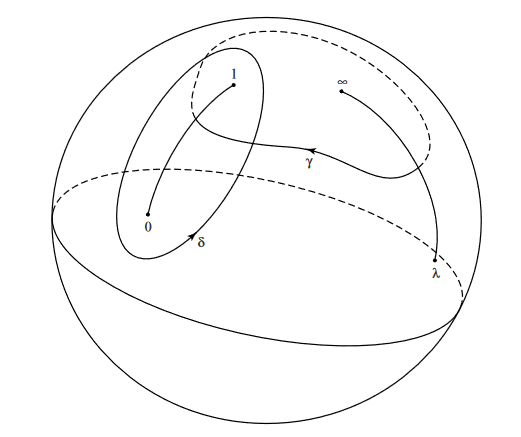
\includegraphics[scale=0.25]{fig1.png}
\end{center}
Then, gluing these two sheets together we get $\cE_\lambda$
\begin{center}
    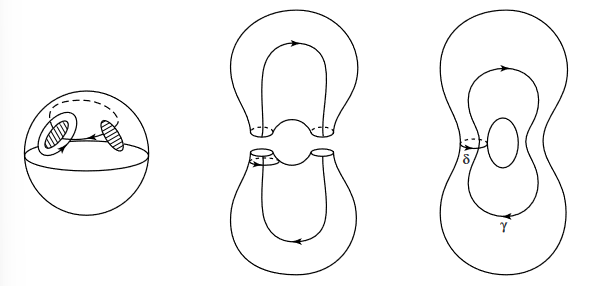
\includegraphics[scale=0.4]{fig2.png}
\end{center}
which is a torus! The interesting cohomology groups for us will be $H^1$, since there isn't anything to say about the Hodge structures in degree 0 or 1---a Hodge structure of weight 0 is boring, and since each $\cE_\lambda$ is a complex torus, $H^2\cong \C$ has to just be $H^{1,1}$, otherwise our dimension would be too high.

So, we pick curves which represent a homology basis of $H_1$, choosing orientations so that $\delta \cdot \gamma = 1$. We also get a dual basis $\delta^*,\gamma^*$ for cohomology.

Now, for a nearby choice of $\lambda$, the essentially the same choice of $\delta,\gamma$ in $\P^1$ will give the identifications of (co)homology. So locally,
\[R^1\pi_*\underline{\C} = \C\delta \oplus \C\gamma\]

\subsection{Hodge filtration of vector bundle.}

We define the form
\[\omega = \frac{dx}{y} = \frac{dx}{\sqrt{x(x-1)(x-\lambda)}}\]
on our family $\cX$, which when restricted to each $\cE_\lambda$ is holomorphic and therefore closed. This gives us a section of our vector bundle $\bH^1$ by
\[\lambda \longmapsto [\omega_\lambda]\]
where $\omega_\lambda$ denotes the restriction to the fiber $\cE_\lambda$. Since $\omega_\lambda$ is holomorphic, we will have
\[[\omega_\lambda] \in H^{1,0}(X_\lambda).\]
We would like to say that $\cF^1 = \cO_X \cdot [\omega_\lambda]$, but we need to check that $[\omega_\lambda]\neq 0$ for any $\lambda$.

We are trivializing our bundle $\bH^1$ by $\delta^*,\gamma^*$, so in these coordinates we can write
\[[\omega_\lambda] = \delta^*\int_\delta \omega_\lambda + \gamma^* \int_\gamma \omega_\lambda.\]
Denote these integrals by $A=A(\lambda)$ and $B=B(\lambda)$ respectively, and we want to show at least one is nonzero. To do this, we show
\[[\omega]\smile [\overline{\omega}] = (A\overline{B}-B\overline{A})\delta^* \smile \gamma^* = -2i\Im(B\overline{A})\delta^* \smile \gamma^*\]
is nonzero. On one hand,
\[i\int_{\cE} \omega \wedge \overline{\omega} = 2\Im(B\overline{A}),\]
(up to a positive scalar multiple) because $\omega^*\smile \gamma^*$ is the orientation.

On the other hand, since $\omega$ is holomorphic, it is locally given by $\omega=fdz$, so
\[\omega \wedge \overline{\omega} = |f|^2 dz\wedge d\overline{z} = -2i|f|^2 dx\wedge dy,\]
so
\[i\omega\wedge \overline{\omega} = 2|f|^2 dx\wedge dy \geq 0,\]
so $i\int\omega\wedge\overline{\omega}$ is positive and in particular nonzero.

\subsection{Gauss-Manin Derivative}

Now, we'd like to see that our Hodge structure on de Rham cohomology actually varies as we vary $\lambda$. To see this, we compute the derivative of $[\omega_\lambda]$ with respective to the Gauss-Manin connection, and see that we get something nonzero.

As per the definition,
\[\nabla [\omega_\lambda] = dA(\lambda) \delta^* + dB(\lambda) \gamma^*,\]
since the $\delta^*,\gamma^*$ provide the local trivialization. Locally, we can think of $\delta,\gamma$ as fixed curves in $\P^1$, against which we integrate the form $\omega_\lambda$ which varies with $\lambda$. In this case, for example,
\begin{align*}
    dA(\lambda) &= \frac{\partial}{\partial\lambda} A(\lambda) d\lambda\\
    &= \left(\pdv{}{\lambda} \int_{\delta} \frac{dx}{\sqrt{x(x-1)(x-\lambda)}}\right) d\lambda\\
    &= \left(\int_\delta \pdv{}{\lambda} \frac{1}{\sqrt{x(x-1)(x-\lambda)}} dx\right) d\lambda\\
    &= \left(\int_\delta \frac{dx}{2\sqrt{x(x-1)(x-\lambda)^3}} \right) d\lambda
\end{align*}
and similarly for $dB(\lambda)$. So, we see that $\nabla [\omega_\lambda] = [\omega_\lambda'] \otimes d\lambda$, where
\[\omega_\lambda' = \frac{dx}{2\sqrt{x(x-1)(x-\lambda)^3}}.\]
This doesn't actually make sense at first glance---this form has a pole at $\lambda$, but it turns out the residue is 0, so by the Gysin sequence, this form represents a cohomology class on all of $\cE_\lambda$: For a Riemann surface $S$ and a discrete subset $A$, we have
\[0 \to H^1(S) \to H^1(S\setminus A) \xrightarrow{\mathrm{res}} H^0(A) \to H^0(S) \to 0,\]
which is obtained from the LES of the pair $(S,S-A)$ and doing Poincar\'e duality.

Now, one can show $\nabla [\omega_\lambda] = [\omega_\lambda']\otimes d\lambda$ is nonzero by reducing to a residue integral calculation.

\subsection{Monodromy Representation}

Finally, we compute the monodromy representation
\[\rho: \pi_1(\P^1\setminus\{0,1,\infty\}) \to \GL(\C^2)\]
associated to our local system $R^1\pi_* \underline{\C}$. First, the fundamental group of our base space is generated by the following loops $a,b$:
\begin{center}
    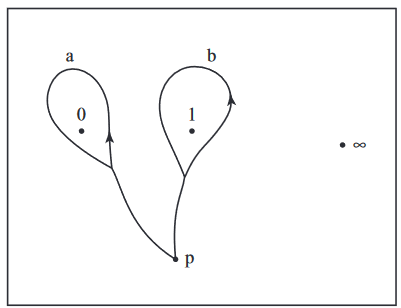
\includegraphics[scale=0.5]{fig3.png}
\end{center}
So, we have to compute the image of $a$ and $b$. Let's compute $\rho(a)$. This is done by going around $a$ at small timesteps so that our local system $R^1\pi_* \underline{\C}$ identifies $H^1(\cE_{\lambda_k}; \C)$ with $H^1(\cE_{\lambda_{k+1}};\C)$, and then to compose these identifications until we potentially get something nontrivial when doing the entire loop. Now, these cohomologies are identified by the diffeomorphisms coming from flowing along the base space, as per the proof of Ehresmann. So, our final isomorphism $\tau^\alpha: H^1(\cE_{p};\C) \to H^1(\cE_{p};\C)$ will be given by (the inverse of) the induced map from the diffeomorphism which is flowing around the entire loop of $a$.

Practically, pick a small circle $S^1$ around $0$, and give it the CW vector field $\pdv{}{\theta}$, which we lift upstairs. Let $g_t$ be the time $t$ map of the flow. Then, $\rho(a)$ will be given by (the inverse of)
\[g_{2\pi}^*: H^1(\cE_p, \C) \to H^1(\cE_p, \C).\]

To compute these, we first choose new branch cuts to make it more convenient. We have the following picture:
\begin{center}
    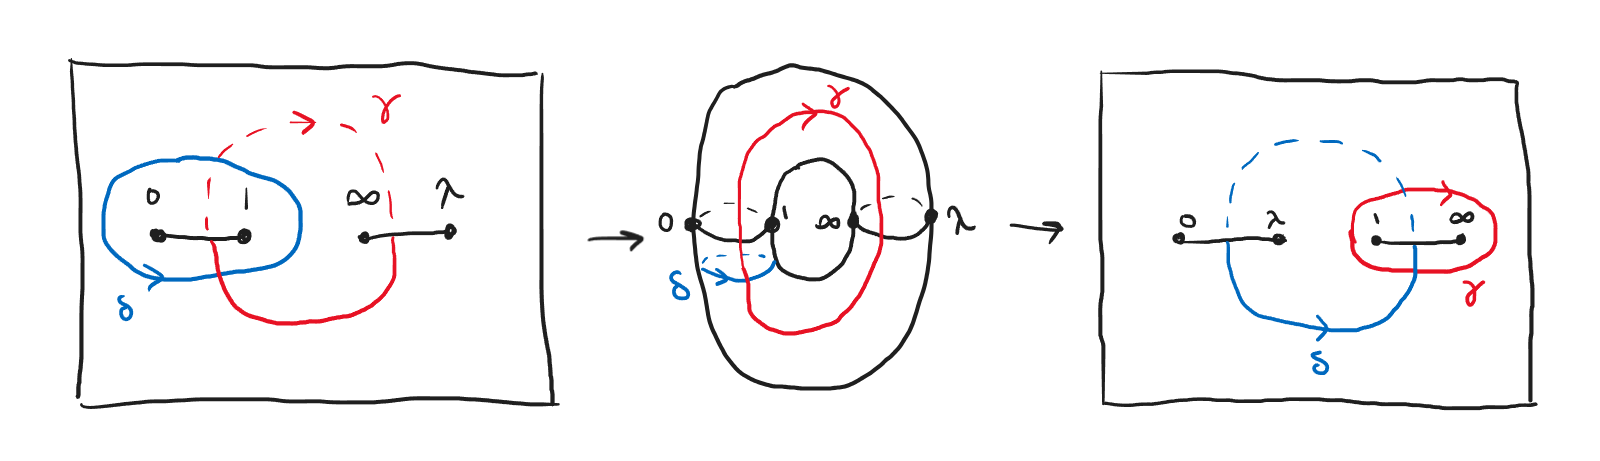
\includegraphics[scale=0.4]{fig4.png}
\end{center}
Now, we draw the following steps:
\begin{center}
    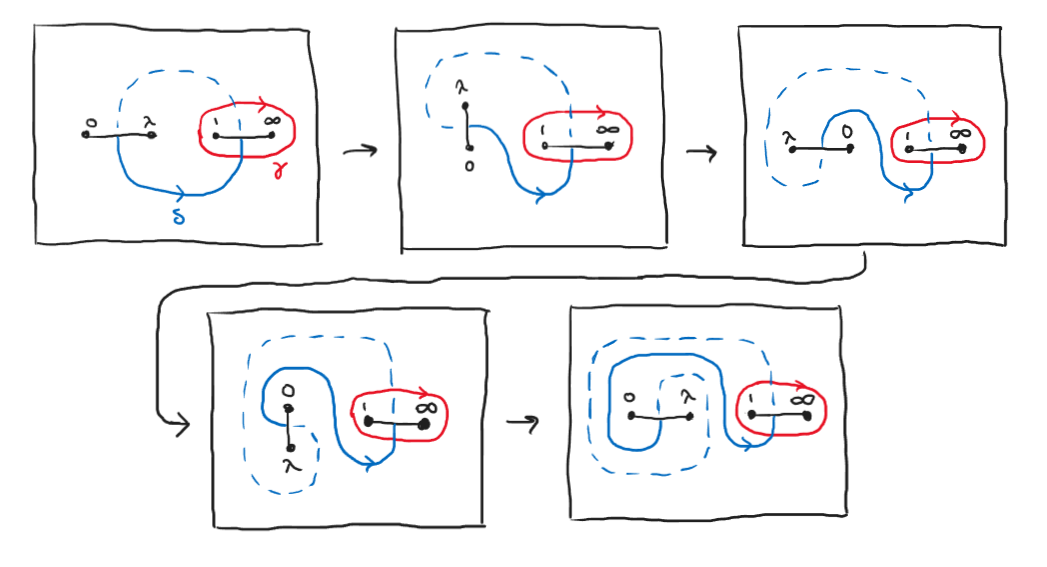
\includegraphics[scale=0.6]{fig5.png}
\end{center}
We relabel the ``new'' $\delta,\gamma$ by $\delta',\gamma'$, and we want to understand how they have transformed via the flow. So, we write $\delta',\gamma'$ in terms of our old basis, by computing them under $\delta^*, \gamma^*$. As usual in Poincar\'e duality, cohomology classes are pairings/intersections with homology classes of the complementary dimensions. This tells us that
\[\delta^*(\alpha) = \alpha \cdot \gamma, \qquad \gamma^*(\alpha) = \delta \cdot \alpha,\]
so we compute using the following picture:
\begin{center}
    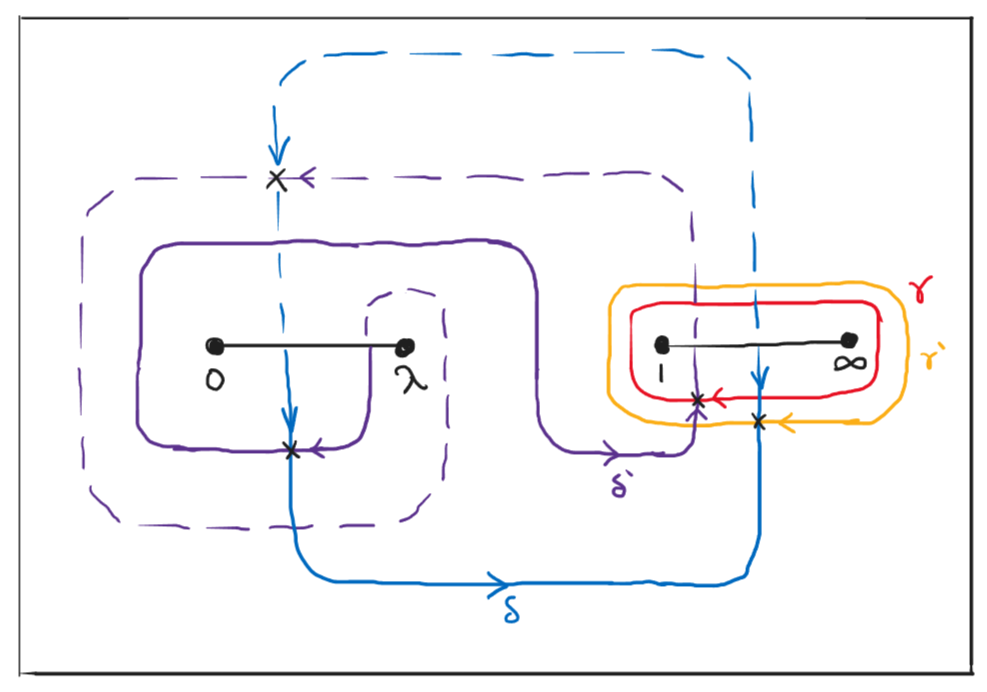
\includegraphics[scale=0.5]{fig6.png}
\end{center}
giving us
\begin{align*}
    \delta' &= \delta - 2\gamma\\
    \gamma' &= \gamma,
\end{align*}
so we see that, represented in the basis $\{\delta,\gamma\}$
\[(g_{2\pi})_* = T = \begin{bmatrix}
    1 & 0\\
    -2 & 1
\end{bmatrix},\]
so
\[\rho(a) = (T^*)^{-1} = \begin{bmatrix}
    1 & 2\\
    0 & 1
\end{bmatrix}.\]
Similar computations should tell us (apparently?)
\[\rho(b) = \begin{bmatrix}
    1 & 0\\
    -2 & 1
\end{bmatrix},\]
which determines our representation $\rho$.

\nocite{*} % Include all references in refs.bib regardless of whether they are referenced or not
\bibliographystyle{plain} % We choose the "plain" reference style
\bibliography{2023spring/variations_of_hodge/variations_of_hodge_refs} % Entries are in the refs.bib file

\end{document}